% $RCSfile$
% $Revision$
% $Date$
% $Source$
%
%
% ---------------------------------------------------------------------------
% TODO:
%
% FINAL READ 
% - check for consistent tense
% - query replace: ai2tv -> $\mathrm{AI}^2$TV
% - spell check
%
%
% ---------------------------------------------------------------------------
% This is "sig-alternate.tex" V1.3 OCTOBER 2002
% This file should be compiled with V1.6 of "sig-alternate.cls" OCTOBER 2002
%
% This example file demonstrates the use of the 'sig-alternate.cls'
% V1.6 LaTeX2e document class file. It is for those submitting
% articles to ACM Conference Proceedings WHO DO NOT WISH TO
% STRICTLY ADHERE TO THE SIGS (PUBS-BOARD-ENDORSED) STYLE.
% The 'sig-alternate.cls' file will produce a similar-looking,
% albeit, 'tighter' paper resulting in, invariably, fewer pages.
%
% ---------------------------------------------------------------------------
% This .tex file (and associated .cls V1.6) produces:
%       1) The Permission Statement
%       2) The Conference (location) Info information
%       3) The Copyright Line with ACM data
%       4) NO page numbers
%
% as against the acm_proc_article-sp.cls file which
% DOES NOT produce 1) thru' 3) above.
%
% Using 'sig-alternate.cls' you have control, however, from within
% the source .tex file, over both the CopyrightYear
% (defaulted to 2002) and the ACM Copyright Data
% (defaulted to X-XXXXX-XX-X/XX/XX).
% e.g.
% \CopyrightYear{2003} will cause 2002 to appear in the copyright line.
% \crdata{0-12345-67-8/90/12} will cause 0-12345-67-8/90/12 to appear in the
%  copyright line.
%
% ---------------------------------------------------------------------------
% This .tex source is an example which *does* use
% the .bib file (from which the .bbl file % is produced).
% REMEMBER HOWEVER: After having produced the .bbl file,
% and prior to final submission, you *NEED* to 'insert'
% your .bbl file into your source .tex file so as to provide
% ONE 'self-contained' source file.
%
% ================= IF YOU HAVE QUESTIONS =======================
% Questions regarding the SIGS styles, SIGS policies and
% procedures, Conferences etc. should be sent to
% Adrienne Griscti (griscti@acm.org)
%
% Technical questions _only_ to
% Gerald Murray (murray@acm.org)
% ===============================================================
%
% For tracking purposes - this is V1.3 - OCTOBER 2002
\documentclass{sig-alternate}
\usepackage{url}

\begin{document}
%
% --- Author Metadata here ---
\conferenceinfo{ACM-MM 2004}{New York, NY USA}
%\CopyrightYear{2001}
% Allows default copyright year (2000) to be over-ridden - IF NEED BE.

%\crdata{0-12345-67-8/90/01}
% Allows default copyright data (0-89791-88-6/97/05) to be over-ridden - IF NEED BE.
% --- End of Author Metadata ---

\title{Optimizing Quality for Collaborative Video Viewing}
%% \title{Alternate {\ttlit ACM} SIG Proceedings Paper in LaTeX
%% Format\titlenote{(Produces the permission block, and
%% copyright information). For use with
%% SIG-ALTERNATE.CLS. Supported by ACM.}}
%% \subtitle{[Extended Abstract]
%% \titlenote{A full version of this paper is available as
%% \textit{Author's Guide to Preparing ACM SIG Proceedings Using
%% \LaTeX$2_\epsilon$\ and BibTeX} at
%% \texttt{www.acm.org/eaddress.htm}}}
%
% You need the command \numberofauthors to handle the "boxing"
% and alignment of the authors under the title, and to add
% a section for authors number 4 through n.
%
% Up to the first three authors are aligned under the title;
% use the \alignauthor commands below to handle those names
% and affiliations. Add names, affiliations, addresses for
% additional authors as the argument to \additionalauthors;
% these will be set for you without further effort on your
% part as the last section in the body of your article BEFORE
% References or any Appendices.

\numberofauthors{4}
%
% You can go ahead and credit authors number 4+ here;
% their names will appear in a section called
% "Additional Authors" just before the Appendices
% (if there are any) or Bibliography (if there
% aren't)

% Put no more than the first THREE authors in the \author command
\author{
%
% The command \alignauthor (no curly braces needed) should
% precede each author name, affiliation/snail-mail address and
% e-mail address. Additionally, tag each line of
% affiliation/address with \affaddr, and tag the
%% e-mail address with \email.
\alignauthor Dan Phung\\
       \affaddr{Computer Science Department}\\
       \affaddr{Columbia University}\\
       \affaddr{New York City, New York}\\
       \email{phung@cs.columbia.edu}
\alignauthor Giuseppe Valetto\\
       \affaddr{Computer Science Department}\\
       \affaddr{Columbia University}\\
       \affaddr{New York City, New York}\\
       \affaddr{and Telecom Italia Lab}\\
       \affaddr{Turin, Italy}
       \email{valetto@cs.columbia.edu}
\alignauthor Gail Kaiser \\
       \affaddr{Computer Science Department}\\
       \affaddr{Columbia University}\\
       \affaddr{New York City, New York}\\
       \email{kaiser@cs.columbia.edu}
}
\additionalauthors{Additional authors: Suhit Gupta {\texttt{suhit@columbia.cs.edu}}}
\date{\parbox[b][0ex]{0em}{\hspace*{-12.5em}\raisebox{37ex}{\fbox{For
submission to \emph{ACM-MM 2004}, due 12:00 AM EDT: April 05, 2004.}}}}
% \date{05 April 2004}
\maketitle

\begin{abstract}
The increasing popularity of distance learning and online courses has
highlighted the lack of collaborative tools for student groups.  In
addition, the introduction of lecture videos into the online
curriculum has drawn attention to the disparity in the network
resources used by the students.  We present an architecture and
adaptation model called $\mathrm{AI}^2$TV (Adaptive Internet
Interactive Team Video), a system that allows geographically dispersed
participants, possibly some or all disadvantaged in network resources,
to collaboratively view a video in synchrony.  $\mathrm{AI}^2$TV
upholds the invariant that each participant will view semantically
equivalent content at all times. Video player actions, like play,
pause and stop, can be initiated by any of the participants and the
results of those actions are seen by all the members.  These features
allow group members to review a lecture video in tandem to facilitate
the learning process.  We employ an autonomic (feedback loop)
controller that monitors clients' video status and adjusts the quality
of the video according to the resources of each client.  We show in
experimental trials that our system can successfully synchronize video
for distributed clients while at the same time optimizing the video
quality, given actual (fluctuating) bandwidth, by adaptively adjusting
	       the quality level for each participant.
\end{abstract}

% A category with the (minimum) three required fields
\category{C.2.4}{Distributed Systems}{Client/server, Distributed applications}
\category{D.2.8}{Software Engineering}{Metrics -- performance measures}
\category{H.5.1}{Information Interfaces and Presentation}{Multimedia Information Systems}
\category{H.5.3}{\\Group and Organization Interfaces}{Computer-\\supported cooperative work, Synchronous interaction}
\category{K.3.1}{Computer Uses In Education}{Collaborative learning, Distance learning}

\terms{ALGORITHMS, MEASUREMENT, PERFORMANCE, EXPERIMENTATION, HUMAN
FACTORS}

\keywords{Synchronized Collaborative Video, Autonomic Controller}

% -------------------------------------------------- %
% FIGURES AT THE FRONT
% -------------------------------------------------- %
%% \begin{figure}
%%   \centering
%%   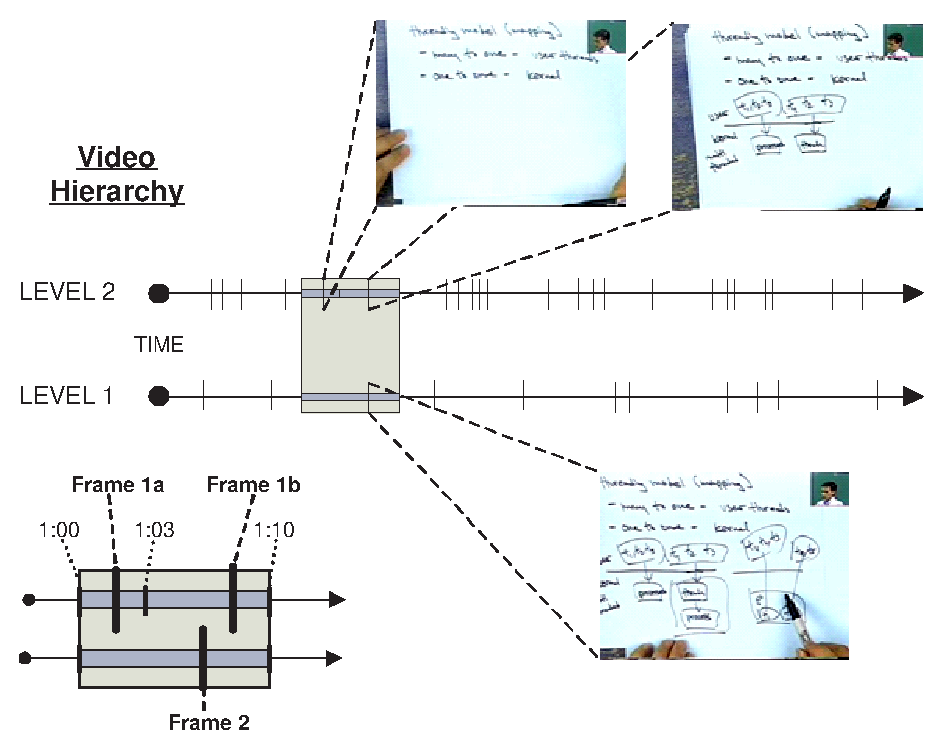
\epsfig{file=vidframes.eps, width=8cm}
%%   \caption{Semantic video compression hierarchy.}
%%   \label{vidframes}
%% \end{figure} 

%% \begin{figure}
%%   \centering
%%   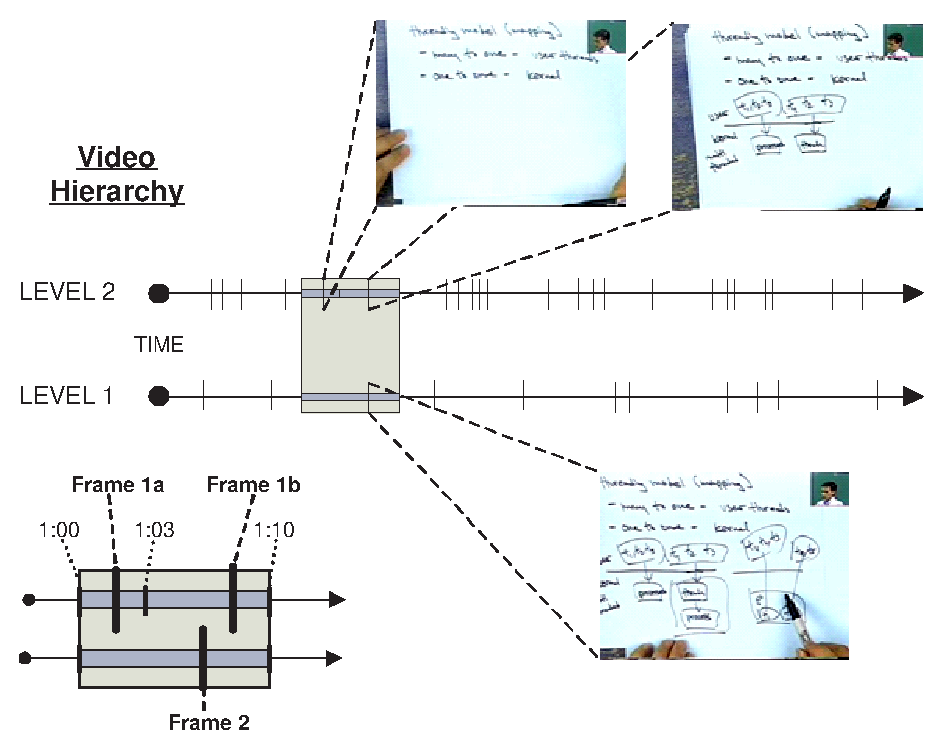
\epsfig{file=vidframes.eps, width=8cm}
%%   \caption{Semantic video compression hierarchy.}
%%   \label{vidframes}
%% \end{figure} 

%% \begin{figure}
%%   \centering
%%   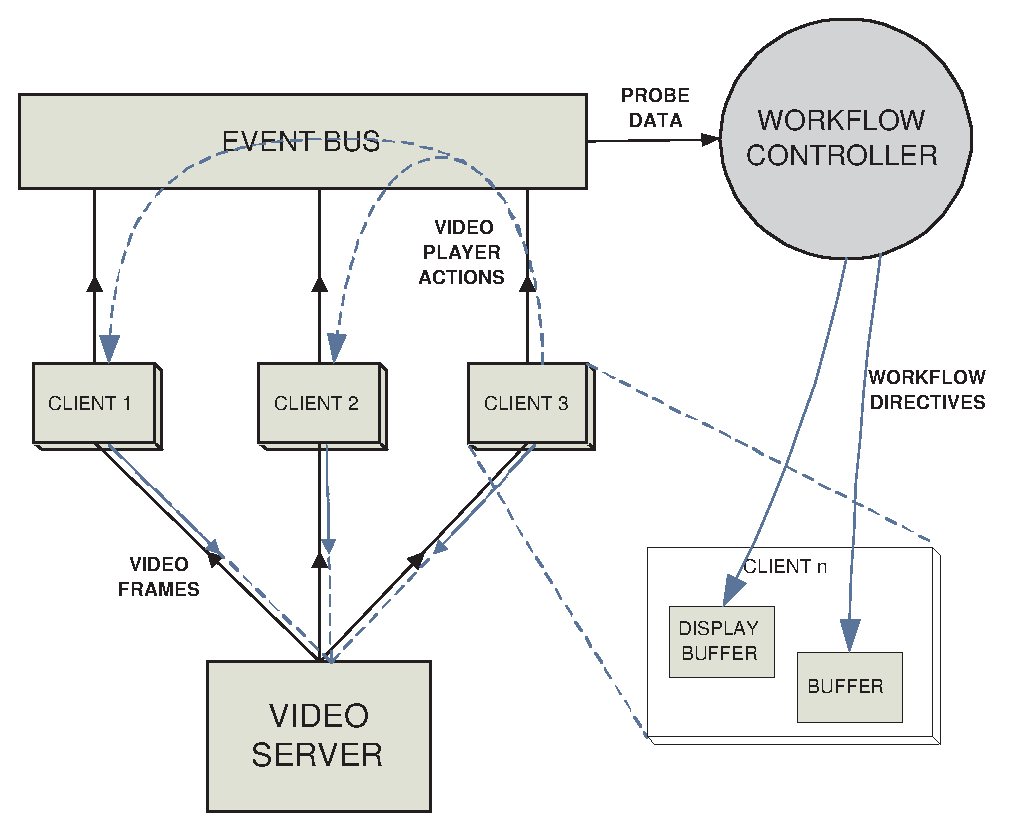
\epsfig{file=ai2tvarch.eps, width=8cm}
%%   \caption{ai2tv Architecture}
%%   \label{ai2tv_arch}
%% \end{figure}


%% \begin{figure}
%%  \centering
%%  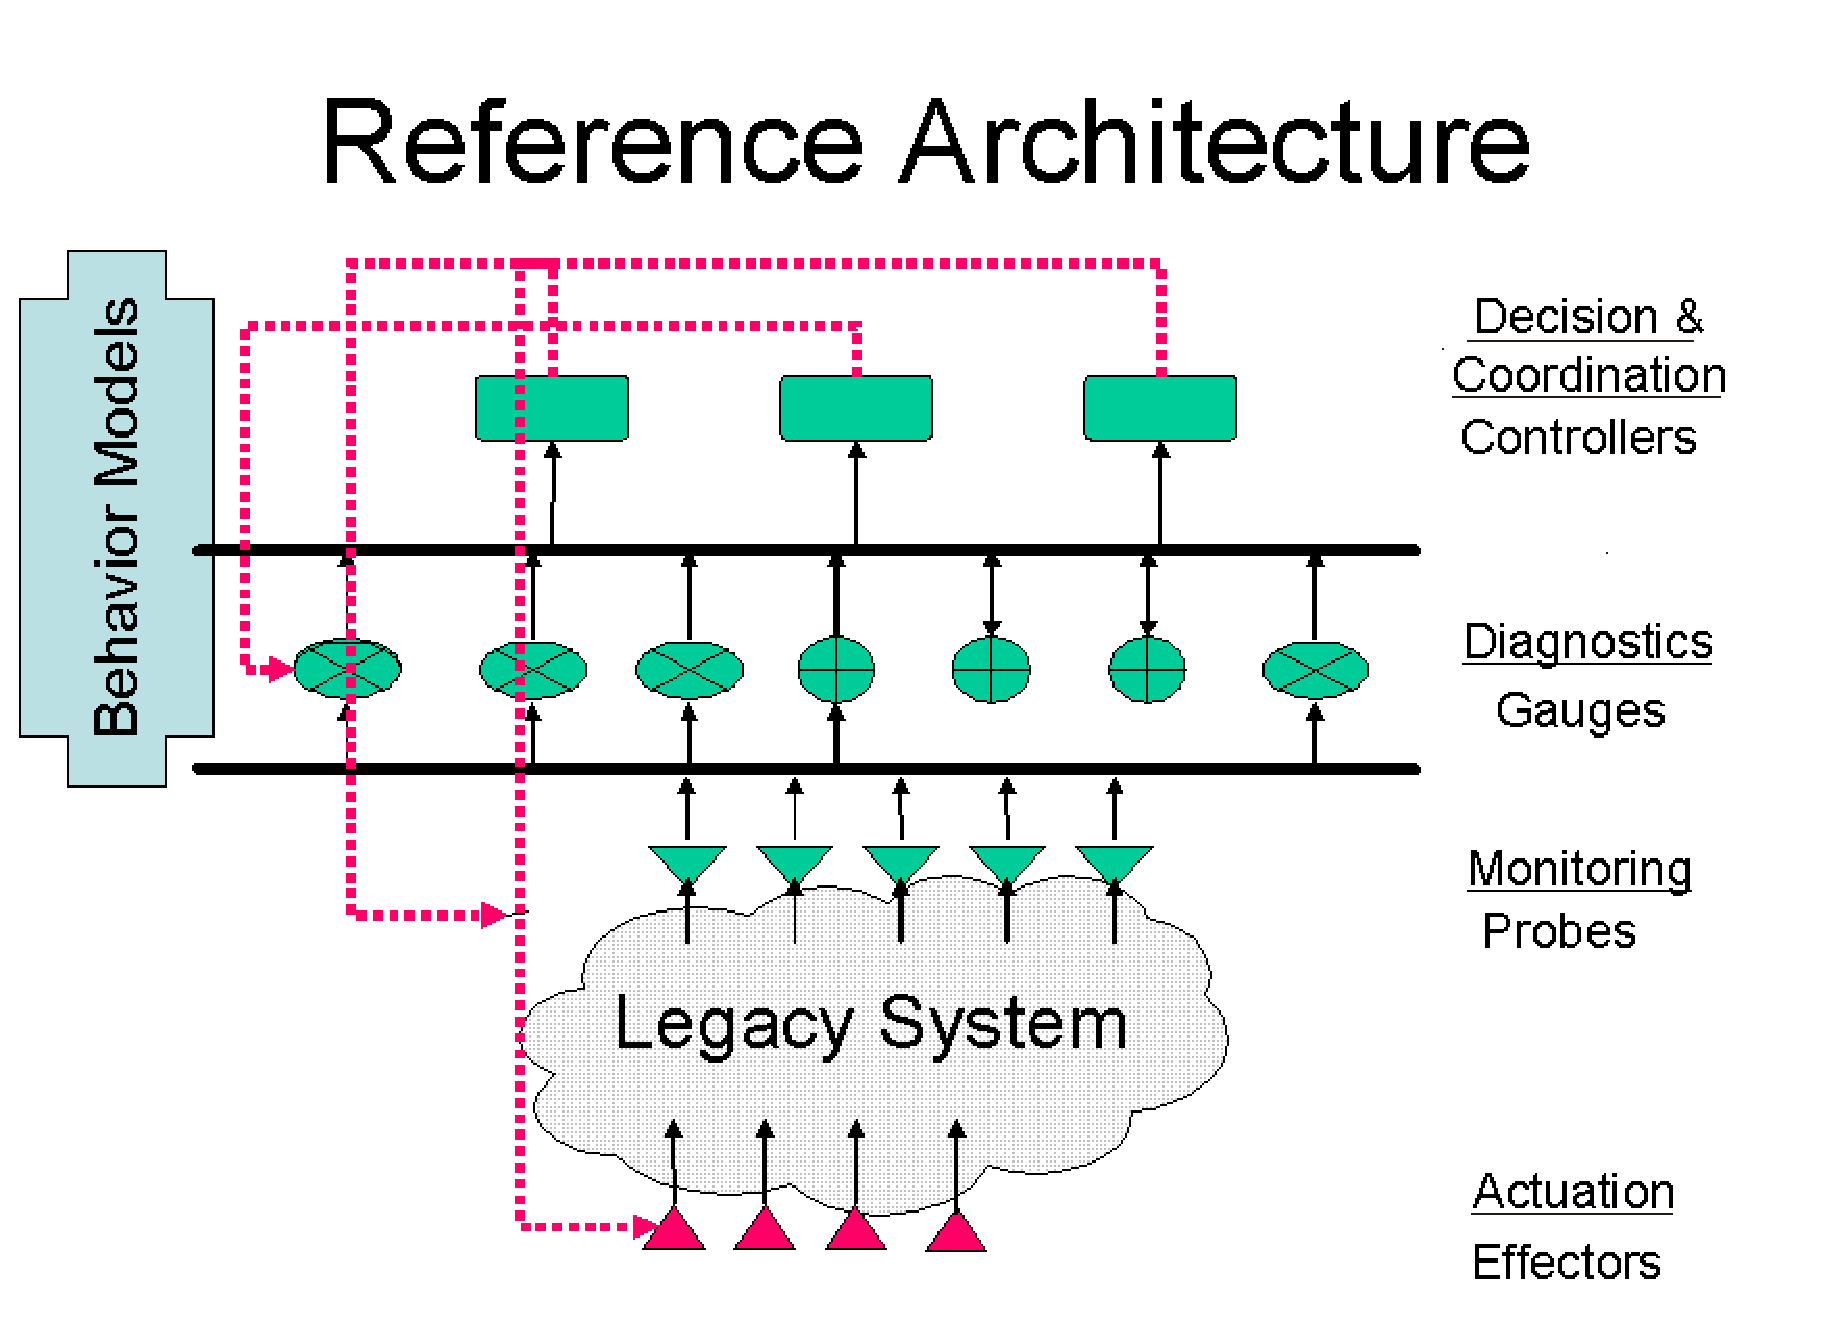
\epsfig{file=refarch.eps, width=8cm}
%%   \label{refarch}
%%  \caption{Conceptual Reference Architecture}
%% \end{figure}


%% \begin{figure} 
%%   \centering
%%   \hspace*{-5mm}
%%   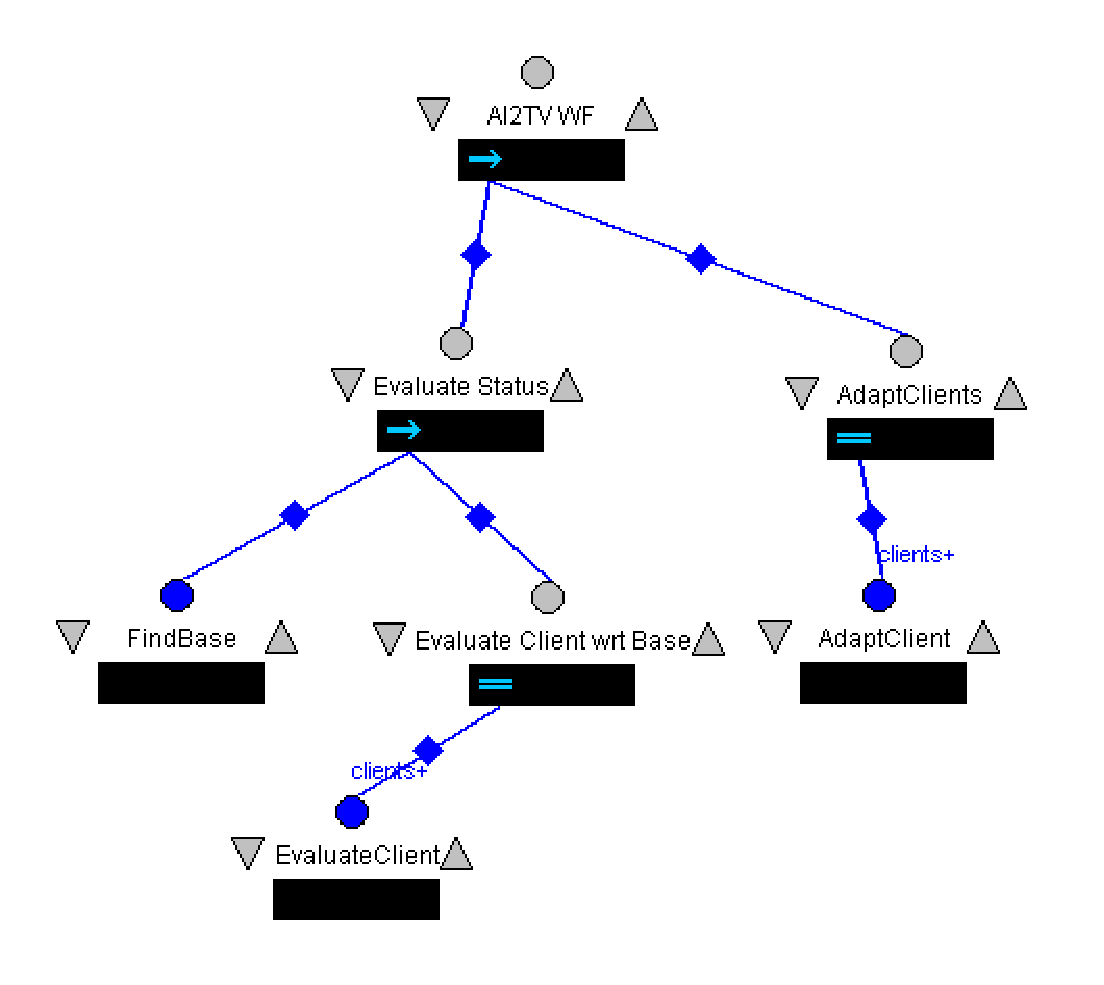
\epsfig{file=ljil.eps, width=8cm}
%%   \caption{Workflow diagram }
%%   \label{ljil}
%% \end{figure}


% -------------------------------------------------- %


% tech report number CUCS-009-04
\section{Introduction}
The increasing popularity of online courses is causing the educational
system to shift away from the conventional practice of only offering
on-campus lecture based courses \cite{BELLER,DOE}.  These online
courses attract a high number of non-traditional working students
because the course work can be scheduled according to the scheduling
needs of each student \cite{BURGESS}.  In addition, online courses
allow students from any region to enroll, leading to a geographically
diverse student population.

To cater to the growing number of online students, universities have
begun taping on-campus course lectures and providing them to
off-campus students \cite{CVN,SCPD}.  This practice introduces the
term of distanced learning to describe students enrolled in a local
program yet attending the courses off-campus.  With the addition of
lecture videos to the available online materials, online students have
access to a greater wealth of information, yet online universities
also have a more complex set of student needs to fulfill.

Traditionally, the courses intended for online students are geared
towards individual learning practices.  The introduction of a whole
new set of courses from on-campus lectures introduced courses that are
sometimes designed for group work.  Because these classes are attended
by both on-campus and off-campus students, the students need tools
that allow group collaboration among a set of remote participants.
Support of synchronous collaboration remains a major concern in
courses where group work is encouraged \cite{WELLS}, yet there are few
educational tools that allow synchronous collaboration across a group
of online students \cite{BURGESS}.  The educational tools commonly
provided for online students are accessed through a personalized Web
portal \cite{PHOENIX,CAPELLA}, which does not provide explicit tools
for group work.

$\mathrm{AI}^2$TV contributes to the area of synchronous collaboration
support, and more specifically, to collaborative video viewing.  In
this scenario, students that are dispersed across different
geographical regions can view a lecture video simultaneously and in a
synchronized manner.  Within a video session, participants can play,
pause, stop and go to certain sections in the video synchronously as a
group.  Therefore a WYSIWIS (What You See Is What I See) invariant is
upheld for all participants.  Note that this invariant applies to
semantic equivalence and not identical video frames.
$\mathrm{AI}^2$TV provides the ability for a group of students to
review a lecture video so that if a participant has a question about a
certain topic, he/she can pause the video and ask questions to other
participants about the material and be assured that all the
participants are referencing the same material.  

% - motivate the use of video as distributed collaboration tool

The erratic nature of network traffic imposes a significant obstacle
to the problem of providing the group review of video across the
Internet.  Viewing video on the Internet requires relatively high
bandwidth resources and lossy network connections can lead to missing
video content.  Furthermore, the differences of network and computing
resources available to dispersed users in the same collaboration group
can be very significant.  Collaborative video viewing poses a twofold
problem: on the one hand, it is mandatory to keep all users
synchronized with respect to the content they are supposed to see at
any moment during play time; on the other hand, it is important to
provide each individual user with a frame rate that is optimized with
respect to the user's available resources, which may vary during the
course of the video.

% - briefly discuss $\mathrm{AI}^2$TV design and imp
In this paper we present an architecture and adaptation model to
address both of the above problems for collaborative video viewing.
Our approach employs a time based synchronization scheme with an
autonomic controller entity.  The term \textit{autonomic} is borrowed
from IBM to mean a self-managing system that uses software based
closed-loop feedback control\cite{IBM}.  Their terminology applies to
the self-management of data centers whereas our work applies to the
domain of multi-user video synchronization.  The autonomic controller
tunes the working parameters of the client's video player in order to
dynamically adjust the video quality levels of the various users in a
group.  We show that it is possible to synchronize content viewing
across all clients while ensuring an high video quality to each of the
the clients.

% - present rest of paper and summarize achievements
In the rest of this paper, we present the motivating problem and
introduce background research that supports this work.  Next, we
explain in detail the architecture and the approach taken in our
solution within the $\mathrm{AI}^2$TV project.  We then present the
criteria used to evaluate the effectiveness of the approach, together
with the corresponding results, and we finish with related work and a
summary of our contributions.

\section{Motivating problem} \label{background}
% - discuss other projects on multiple client synchronization
The advent of the Internet and the World Wide Web as a major means of
communication has presented the educational community with the
potential for great gains in the realm of accessibility to education
through e-Learning.  A variety of e-Learning applications that support
individual study practices exist, and typically follow the metaphor of
a Web portal where registered users can individually browse class
material or post completed assignments \cite{PHOENIX,CAPELLA}.
Several other applications can be used to provide some level of
support to online educational collaboration, although they may not be
geared specifically towards educational purposes.  Among them, some
are geared towards asynchronous forms of collaboration, (for example
Web-based bulletin boards and discussion groups); others, such as
instant messaging, application and desktop sharing \cite{WEBEX, VNC},
and co-browsing \cite{CAPPS, LIEBERMAN, SIDLER} facilitate mostly the
communicative aspects of synchronous collaboration, such as the
long-distance sharing of ideas and knowledge among their users.
However, there are few tools that provide an on-line study environment
to support synchronous collaborative study practices, such as the
group review of educational material produced for on-line courses
\cite{WELLS}.  For example, Easy Teach and Learn proposes a virtual
classroom architecture that allows multiuser synchronous
participation, but only a simulated version of this system has been
implemented \cite{WALTER}.

% - ai2tv project goals
The work presented in this paper is a part of the $\mathrm{AI}^2$TV
project, a multi-group effort aimed at developing a collaborative
virtual environment for distributed team study.  $\mathrm{AI}^2$TV
differs from many existing approaches that provide educational content
in a networked context because of its explicit focus on the teamwork
aspects of on-line education, and hence on synchronous collaboration.
Within $\mathrm{AI}^2$TV, an important goal is to provide support for
the collaborative use of multimedia content relevant to the work
carried out by a team of users involved in the same project, such as
audio/video recordings of lectures, meetings, workshops and other
informational and educational events.

One of the requirements of the multimedia support within the
$\mathrm{AI}^2$TV virtual environment is the synchronized viewing of
streaming video by all members of a geographically distributed team.
To enforce the metaphor of synchronous collaboration in a virtual
environment and for collaboration to be effective, all team members
must be viewing the same content at all times so that discussion of
the material can be coherent.  Synchronized viewing, however, is
particularly difficult in an Internet context: dispersed team members
may enjoy very diverse connectivity, ranging for example from 56k
modem, to DSL, to cable, to T1 lines.  Moreover, the communication and
computing resources available to each user may widely and quickly vary
in the course of the team work session.

To deal with these constraints, we adaptively control the distribution
and presentation of the multimedia to all team members.  To be usable,
that control must achieve synchronized viewing without unreasonably
constraining the quality of the viewing experience of individual
users; for example, a "worst case scenario" in which the experience of
all members in a team is degraded to match that of the member with the
least resources is not acceptable. On the contrary, any valid solution
must reconcile the mandatory requirement of synchronized viewing with
an efficient use of the resources of individual users.

One solution to the problem of balancing the group synchronization
requirement with the optimization of individual viewing experiences is
to use videos with cumulative layering \cite{MCCANNE}, also known as
scalable coding \cite{LI}.  In this approach, the client software is
instructed to display video content at a quality level appropriate for
that client's resources, which is selected from a hierarchy of several
different encodings or frame rates for that video.

% - describe overview of semantic compression tool used
Either fixed rate or variable rate schemes can be equally employed. In
$\mathrm{AI}^2$TV, we take advantage of a semantic summarization
package that was developed at Columbia University by Liu and Kender
\cite{TIECHENG} which reduces a video to a set of semantically
significant key frames.  That tool operates on MPEG format videos and
outputs sequences of JPG frames, some of which are displayed in figure
\ref{semvid}.  Its semantic compression algorithm profiles video
frames within a sliding time window and selects key frames that have
the most semantic information.  By increasing the size of the window,
a key frame will represent a larger time slice, which means that a
larger window size will produce less key frames as compared to a
smaller window size setting.

\begin{figure}
  \centering
  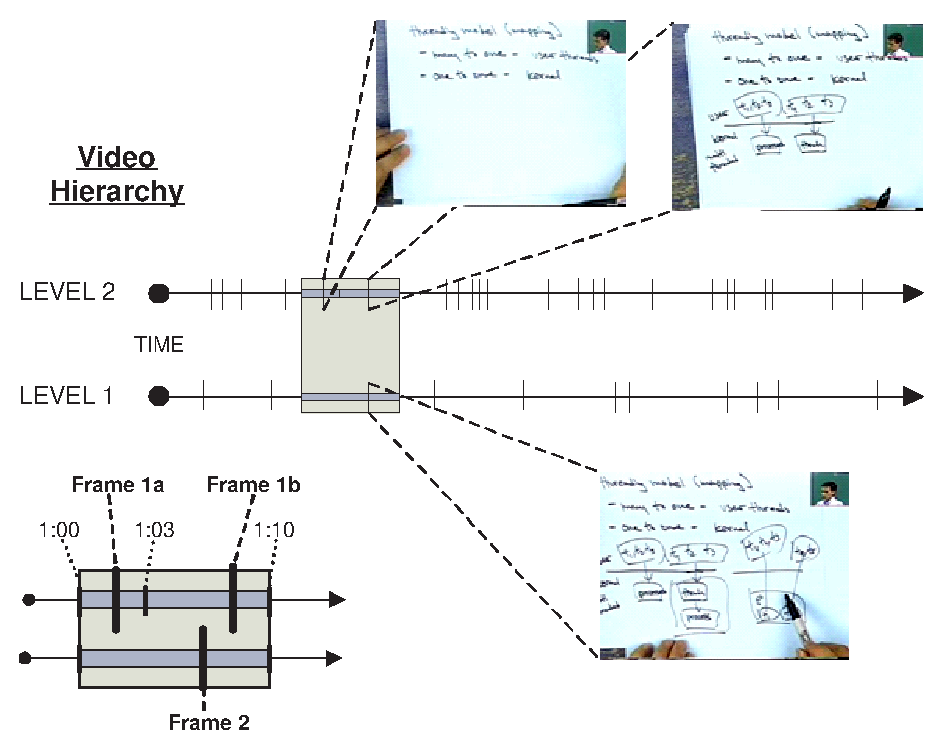
\epsfig{file=vidframes.eps, width=8cm}
  \caption{Semantic Video Scenario}
  \label{sem_video}
\end{figure} 

The semantic compression package is used to produce the layered videos
provided to clients.  A conceptual diagram of a video is shown in
figure \ref{sem_video}.  Note that the semantic compression algorithm
produces a random distribution of key frames, hence the video produced
by the package plays back at a variable frame rate.  The variability
in the frame rate implies that there are pockets of relatively high
frequency semantic change that result in sections in the video that
demand a higher frame rate.  The variable frame rate video adds
complexity to the bandwidth demands of the client yet its semantic
focus ensures that relevant content is unlikely to get lost, which is
a significant property in the context of an educational application.

Also, in figure \ref{sem_video}, the bottom-left in-set shows the
juxtaposition of individual frames from two different quality levels.
Each frame has a representative time interval \texttt{[start:end]}.
For the higher level, Frame 1a represents the interval from 1:00 to
1:03, and Frame 1b represents the interval from 1:04 to 1:10.  For the
lower level, Frame 2 represents the entire interval of 1:00 to 1:10.

Through the use of the $\mathrm{AI}^2$TV video, we can provide
semantically equivalent content to several clients with diverse
resources by adjusting the compression level assigned to each client
while the user is watching the video.  Thus for our purposes,
synchronization of video boils down to showing semantically equivalent
frames for a given time.

To adjust the clients in response to the changing environment, we use
an autonomic controller to maintain the synchronization of the group
of video clients while fine tuning the video quality for each client.
In \cite{RAVAGES}, we proposed the idea of using an autonomic
controller to support group video synchronization and other multimedia
applications.

The autonomic controller remains conceptually separate from the
controlled $\mathrm{AI}^2$TV video system and employs a software based
workflow engine, named Workflakes \cite{ICSE}.  Note that the workflow
used here is software based as opposed to human based workflow
systems.  The use of software based workflow for the specification and
enactment of the plan that coordinates actuators is taken from Wise at
al. \cite{OSTERWEIL} among others.  The Workflakes engine has been
developed for and used in a variety of domains \cite{AMS,ICSE}, in
which it orchestrates the work of software entities to achieve the
fully automated dynamic adaptation of distributed applications.  The
design of the autonomic controller is a part of an externalized
autonomic computing platform proposed by Kaiser \cite{REFARCH}.  In
the context of $\mathrm{AI}^2$TV, Workflakes coordinates the
adjustment of the compression level assigned to each client along the
hierarchy of the $\mathrm{AI}^2$TV video.

% (FIGURE: semantic compression )
% (FIGURE: key frames hierarchy )

\section{Architecture and Adaptation\\ Model}
\subsection{System Architecture}
% Design of a the system in general
Our system involves several major components: a video server, video
clients, an externalized autonomic controller and a common
communications infrastructure, as seen in figure \ref{ai2tv_arch}

\begin{figure}
  \centering
  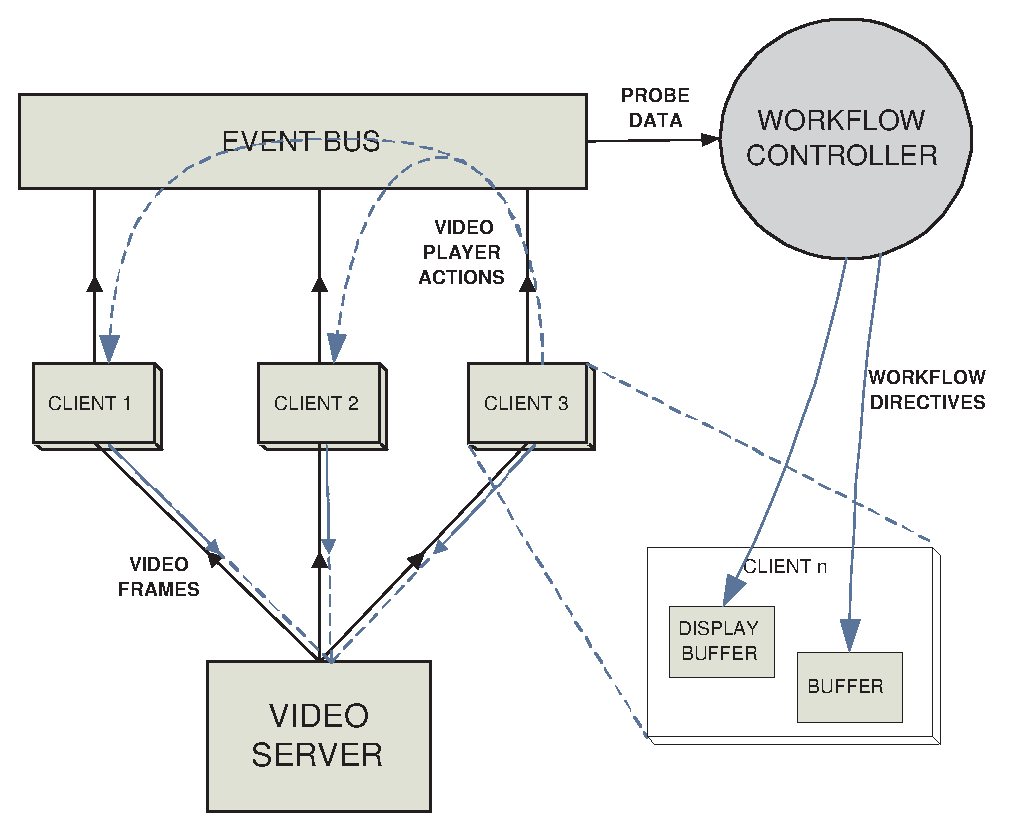
\epsfig{file=ai2tvarch.eps, width=8cm}
  \caption{$\mathrm{AI}^2$TV Architecture}
  \label{ai2tv_arch}
\end{figure}

%(FIGURE: ai2tv synchronization arch)
% video server
The video server provides the educational video content to the clients
for viewing.  The provided content has the form of an
$\mathrm{AI}^2$TV video, i.e., a hierarchy of video versions produced
by running the tool multiple times with settings for different
compression levels, which produces several sets of JPG frames that are
indexed by a frame index file.  The task of the video server is simply
to provide remote download access to the frames and the index file
over HTTP.

% video client
The task of video clients is to acquire video frames, display them at
the correct time, and provide a set of basic video functions.  Taking
a functional design perspective, the client is composed of three major
modules: a video display, a video buffer and manager for fetching and
storing downloaded frames, and a time controller.

The video display renders the JPG frames into a window for display and
provides a user interface for play, pause, goto, and stop.  When any
participant initiates one of these actions, all the other group
members receive the same command, thus all the video player actions
are synchronized.  The video display knows which frame to display by
using the current video time and display quality level to index into
the frame index for the representative frame.  Before trying to render
the frame, it asks the video buffer manager if the needed frame is
available.  The video display also includes a control entity that
enables external entities, like the autonomic controller, to adjust
the current display quality level.

The video buffer and manager constitute the downloading daemon that
continuously downloads frames at a certain level.  It keeps a hash of
the available frames and a count of the current reserve frames (frames
buffered) for each quality level.  The buffer manager also includes a
control hook that enables external entities to adjust the current
downloading quality level.

The time controller's task is to ensure that a common video clock is
maintained across clients.  It relies on NTP \cite{NTP} to synchronize
the system's software clock therefore ensuring a common time base from
which each client can reference for the video clock.  The task of each
then is to play the frames at the correct time and since all the
clients refer to the same time base, then all the clients are showing
semantically equivalent frames.

% autonomic controller
The task of the autonomic controller is to ensure that the clients
within a video session stay synchronized and that each client plays at
its highest attainable quality level.  The controller is a distributed
system, whose design derives from a conceptual reference architecture
for externalized autonomic computing platforms proposed by Kaiser
\cite{REFARCH}, which is shown in figure \ref{refarch}. The
architecture provides an end-to-end closed control loop, in which
sensors attached to a generic (possibly legacy) target system and
continuously collect and send streams of data to gauges.  The gauges
analyze the incoming data streams and respond to conditions that need
adaptation by relaying that information to controllers.  The
controllers coordinate the expression and orchestration of the
workflow needed to carry out the adaptation.  To close the loop,
actuators at the target system effect the needed adjustments under the
supervision of the controller.

%
%(figure of ref arch here). 
%

\begin{figure}
 \centering
 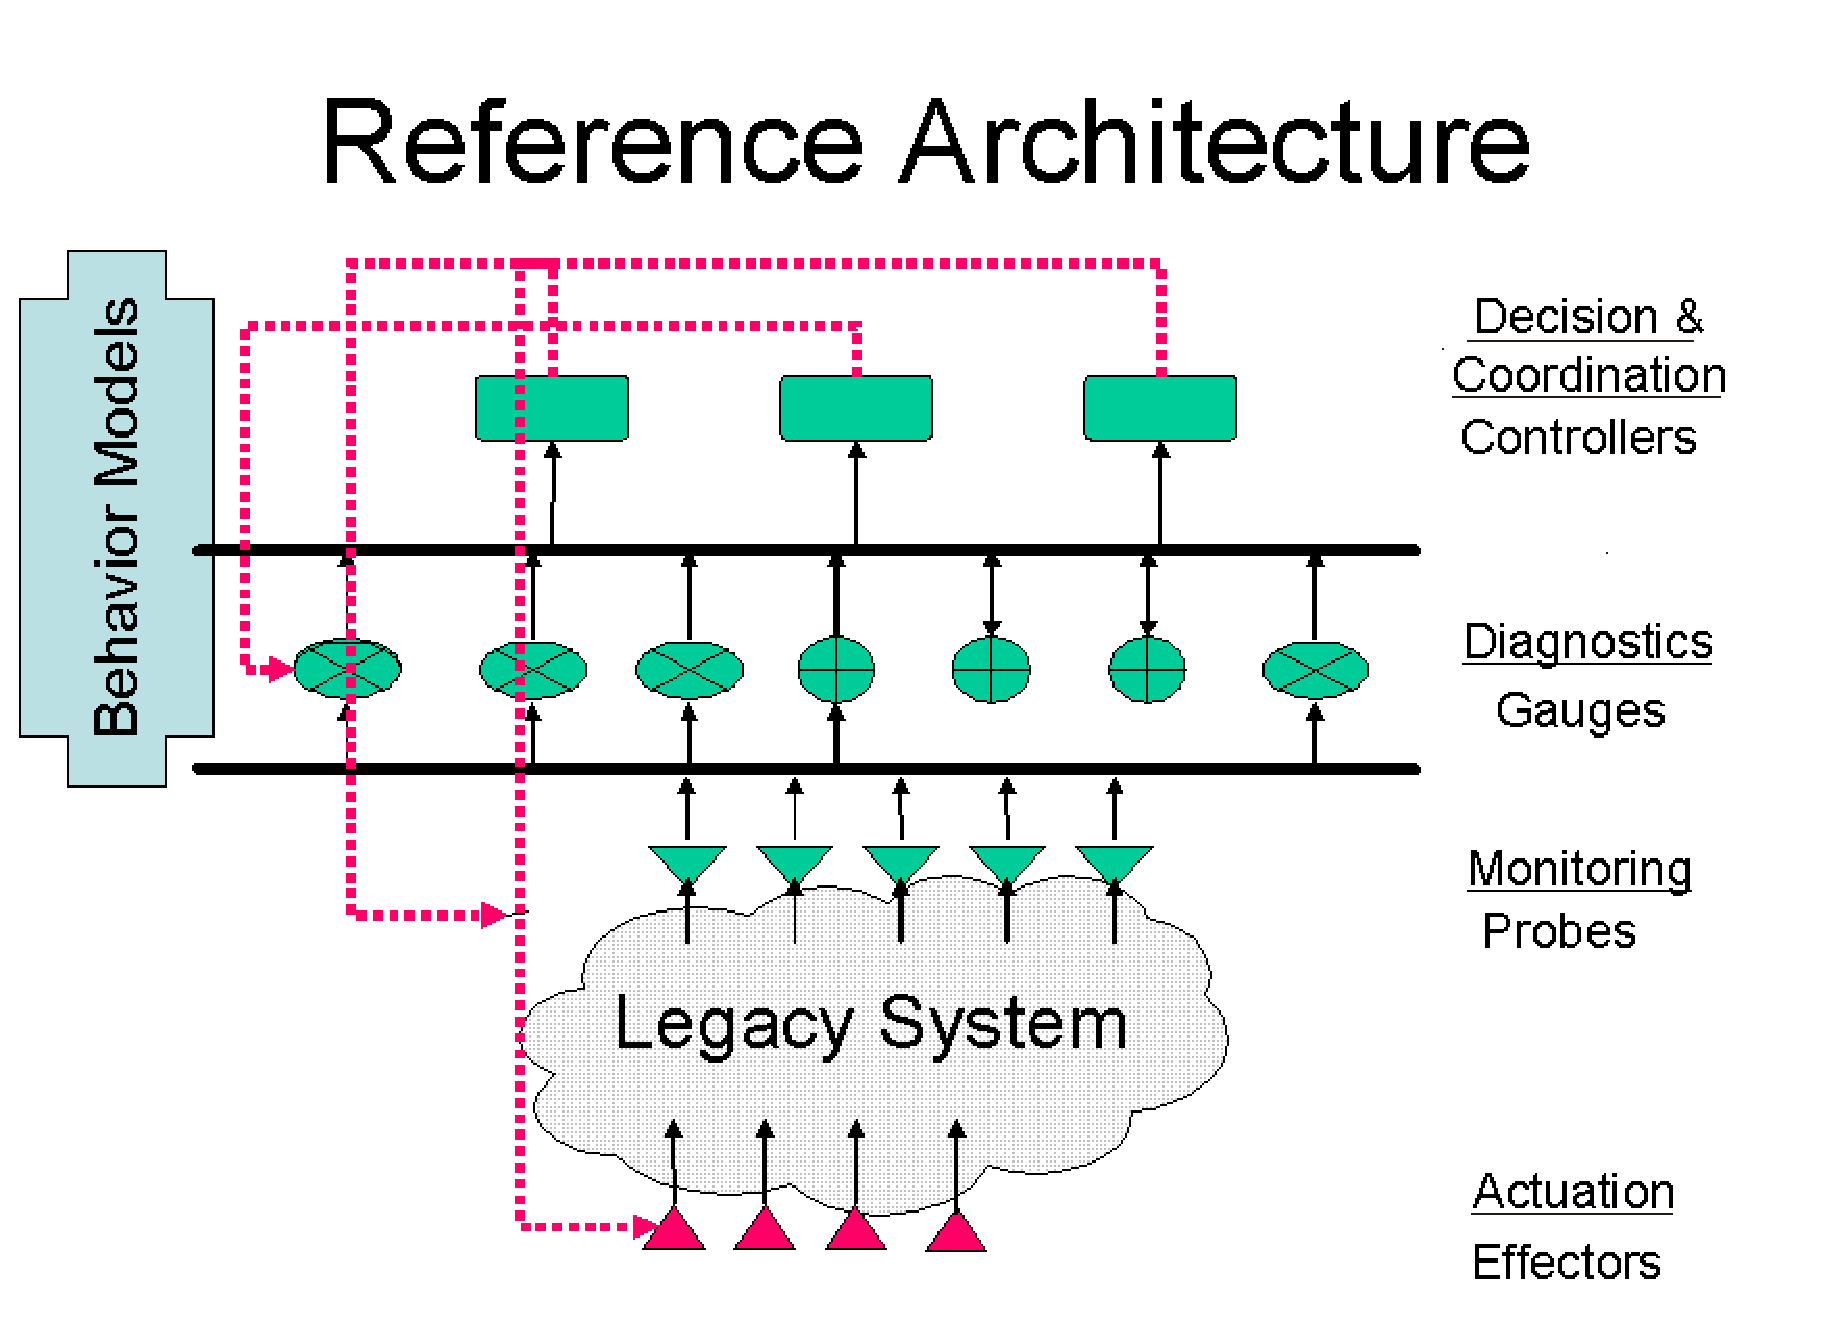
\epsfig{file=refarch.eps, width=8cm}
  \label{refarch}
 \caption{Conceptual Reference Architecture}
\end{figure}


The sensors provide the autonomic controller with data about the
clients such as video display quality level, the buffer quality level,
the buffer reserve frames, the currently displayed frame and the
current bandwidth.  Gauges are embedded together with the coordination
engine for expediency of design and to minimize the communication
latency to it.  They receive the sensor reports from individual
clients, collect them in buckets, similar to the approach in
\cite{MIMAZE}, and pass the bucket data structure to the coordination
engine.  The coordination engine directs the flow of the information
through a predefined workflow plan described in the next section.

During the evaluation of the data, a set of helper functions that are
tailored specifically for the application are used to produce the
triggers for the coordinator.  If a trigger is raised, the
coordination engine enacts an adaptation scheme which is executed on
the end hosts by hooks provided to the actuators by the end systems.

% communications 
The infrastructure used for the communications among the video
clients, as well as between the $\mathrm{AI}^2$TV system and the
autonomic controller is provided by an event bus based on the
publish/subscribe paradigm.  The reason for choosing this
communication model is that it inherently decouples the physical
location of the communicating entities.  Events transmitted onto that
event bus are of three kinds: video player actions, sensor reports and
adaptation directives (see figure \ref{ai2tv_arch}.  Video player
actions pertain to the functionality of the $\mathrm{AI}^2$TV system,
since they represent commands issued on a video client, such as pause,
play or stop, which need to be propagated to all clients in the group
to enforce the same behavior.  All video player actions are time
stamped so that clients can respond to those commands in reference to
the common time base.

\subsection{Adaptation Model}

The adaptation scheme falls into two levels: a higher level data flow,
and a lower level adjustment heuristic.  The former directs the flow
of data through a logical sequence to provide a formal decision
process while the latter provides the criteria as to when to make
certain adjustments.

The higher level logic is shown in figure \ref{ljil}, according to the
Little-JIL graphic workflow specification language \cite{LJIL}.  The
diagram shows the task decomposition hierarchy according to which the
adaptation workflow unfolds.  Note that the evaluation of clients'
state with respect to the group (\texttt{EvaluateClient}) and the
issuing of adaptation directives (\texttt{AdaptClient}) is carried out
as a set of the parallel steps.  Also note that the multiplicity of
those parallel steps is dynamically determined via the number of
entries in the \texttt{client} variable, which maps to a collection of
$\mathrm{AI}^2$TV clients.

%
%add Figure with AI2TV workflow diagram here
%

\begin{figure} 
  \centering
  \hspace*{-5mm}
  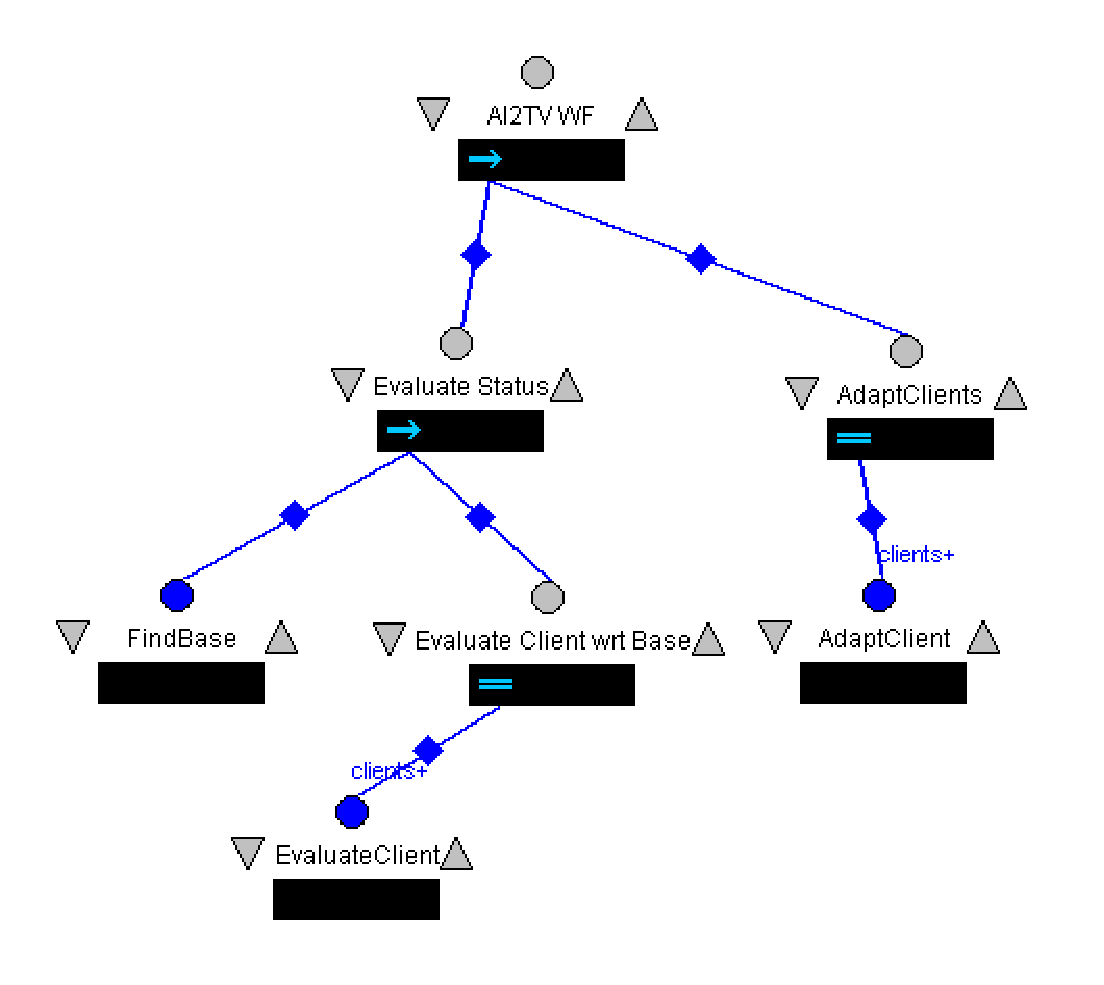
\epsfig{file=ljil.eps, width=8cm}
  \caption{Workflow diagram }
  \label{ljil}
\end{figure}

The adaptation scheme at the lower level falls into two categories:
directives that adjust the client in response to relatively low
bandwidth situations, and those that take advantage of relatively high
bandwidth situations.

In the situation where a client has relatively low bandwidth, the
client may not be able download next frame at the same quality level
in time.  This situation will merit that both the client and the
buffer quality levels are reduced one level. In the case in which the
client is already at the lowest level, the controller will calculate
the next possible frame that it can successfully complete in time - in
order to remain synchronized with the rest of the team - and will ask
the client to jump ahead to that frame.

To take advantage of relatively high bandwidth situations, the buffer
manager will start to accumulate a reserve buffer.  Once the buffer
reaches a threshold value (for example, 10 buffered frames), the
autonomic controller will direct the buffer manager to start fetching
frames a higher quality level.  Once a sufficient reserve is
accumulated also at that higher level, the client is then ordered to
display frames at that quality level.  If the bandwidth drops before
the buffer manager controller can accumulate enough frames in the
higher-level reserve, then the buffer manager is dropped back down one
level.

\section{Implementation} \label{implementation}

For simplicity, we used Java to implement the video client.  It
naively uses the javax.swing package to render the JPG images.  The
autonomic controller, Workflakes, is also Java based and uses Cougaar
\cite{COUGAAR} as the workflow engine.  We used the Little-JIL graphic
workflow specification language to produce the workflow used
\cite{LJIL}.  We chose a content-based publish-subscribe event system,
Siena, as our communication bus \cite{SIENA}.

\section{Evaluation} \label{eval}

We assess our system by evaluating its ability to synchronize the
clients and its ability to adjust the clients video quality.  The
evaluation results presented in this section were computed from a set
of client configurations, specifically 1, 2, 3, and 5 clients running
a video for 5 minutes and probing system state every 5 seconds. The
compression hierarchy we employed has 5 different levels.

For our evaluation, we define a baseline client against which the
performance of our approach can be compared.  A baseline client is a
client whose quality level is set at the beginning of the video and
not changed thereafter.  To define the baseline client, we use a value
that we identify as the average bandwidth per level. This value is
computed by summing the total size in bytes of all frames produced at
a certain compression level and dividing by the total video time.
This value provides the bandwidth needed on average for the buffer
controller to download the next frame on time.  We provide the
baseline client with the needed bandwidth for its chosen level by
using a bandwidth throttling tool (\cite{SHAPERD}) to adjust the
bandwidth to that client from the video server.  Note that using the
average as the baseline does not account for changes in the video
frame rate and fluctuations in network bandwidth, which are situations
in which adaptive control can make a difference.

When carrying out the evaluation, each controller-assisted client is
assigned an initial level in the compression hierarchy and the same
bandwidth as the baseline client for that hierarchy level.  At the end
of each experiment, we record any differences resulting from the
adaptation of the clients' behavior on the part of the autonomic
controller and the behavior of the baseline client, with respect to
synchrony and quality of service (frame rate).

%% To evalute our system, we produced an $\mathrm{AI}^2$TV video that had 5 quality
%% levels.  For a 17 minute video and five different window lengths, the
%% total number of frames are 165, 71, 39, 21, and 13.  Our choice of the
%% relatively low frame rate quality levels was influenced by the goal of
%% the system being used by clients with low bandwidth resources.
 
% the pathetic average frame rates (per minute!!!):
%% 3.399831413 - high
%% 1.46295776
%% 0.806289939
%% 0.434237734
%% 0.268763313 - low

\textit{Evaluating Synchrony}

A major goal of the system is to provide synchronous viewing to all
clients.  To measure the effectiveness of the synchrony, we probe the
clients at periodic time intervals and log the frame currently being
displayed.  This procedure effectively takes a snapshot of the system,
which we can evaluate for correctness.  This evaluation proceeds by
checking whether the frame being displayed at a certain time
corresponds to one of the valid frames at that time, on any arbitrary
level.  We allow any arbitrary level because the semantic compression
algorithm ensures that all frames at a certain time will contain the
same semantic information if the semantic windows overlap.  We score
the system by summing the number of clients not showing an acceptable
frame and normalizing over the total number of clients.  A score of 0
indicates a synchronized system.

Our experiments for the evaluation of synchronization initially
involved groups of clients that were set to begin playing the test
video at different levels in the compression hierarchy, and were
assigned the corresponding baseline bandwidth. In those experiments,
the results show a total score of 0 for all trials. Also,
notwithstanding the variations in the frame rate and/or occasional
fluctuations in the actual bandwidth of the clients, no frames were
missed.  This result demonstrates that the chosen baseline
combinations of compression levels and throttled bandwidths do not
push the clients beyond their bandwidth resource capacity.

We also ran another set of experiments, in which the clients in the
group were assigned more casually selected levels of starting
bandwidths.  This casual selection is representative of a real world
situation, like listening to Internet radio, where users must choose a
desired frame rate to receive.  The user may have been informed that
she is allocated a level of bandwidth from her Internet service
provider, but she may actually be receiving a significantly lower
rate.  We ran experiments first without the aid of the autonomic
controller and then with it. In the former case, clients with
insufficient bandwidth were stuck at the compression level originally
selected, and thus missed an average of 63\% of the needed frames.  In
the latter case, the same clients only missed 35\% of the needed
frames.  These results provide evidence of the benefits of the
adaptive scheme implemented by the autonomic controller.

%% selected, and thus only displayed an average of 37\% of the needed
%% frames.  In the latter case, the same clients received 65\% of the
%% needed frames.  These results provide evidence of the benefits of the
%% adaptive scheme implemented by the autonomic controller.


%% \begin{figure} 
%%   \centering
%%   \hspace*{-5mm}
%%   \epsfig{file=scores.eps, width=9cm}
%%   \caption{Comparison of weighted scores}
%%   \label{scores}
%% \end{figure}

\textit{Evaluating Quality of Service} 

A primary goal of the $\mathrm{AI}^2$TV system is to increase the
video quality for the clients.  With respect to the evaluation of
video quality of services, Liu et. al describes several local metrics
such as frame rate, loss rate, delay jitter, image resolution, and
human spatial-temporal contrast-sensitivity \cite{LIU}.  We do not
address global metrics such as fairness, as described in \cite{LIU}.
For our situation, a higher video quality means a higher frame rate.

To attain a quantitative measure of the quality of service provided by
a client assisted by the autonomic controller, we use a scoring system
relative to the baseline client's quality level.  We give a weighted
score for each level above or below the baseline quality level.  The
weighted score is calculated as the ratio of the frame rate of the two
levels.  So, for example, if a client is able to play at one level
higher then the baseline, and the baseline plays at an average
\texttt{n} fps while the level higher plays at \texttt{2*n} fps, the
given score for playing at the higher level is 2.  The weighted score
is calculated between the computed average frame rates of the chosen
quality levels.  Theoretically, the baseline client should receive a
score of 1.  Note that we formulated this scoring system because other
scoring systems \cite{BAQAI,CORTE,CONWAY2000} measure unrelated
factors such as the synchronization between different streams (audio
and video), image resolution, or human perceived quality, and are not
restricted by the group synchronization requirement.  This restriction
mandates that a scoring system be sensitive to the relative
differences between quality hierarchies.

% qos results
The evaluation of the quality of service experiments shows that the
baseline clients scored a group score of 1 (as expected) while the
clients assisted by the autonomic controller scored a group score of
1.25.  The one-tailed t-score of this difference is 3.01 which is
significant for an $\alpha$ value of .005 (N=17).  This result
demonstrates that using the autonomic controller, we are able to
achieve a significant positive difference in the quality of services.
Note that the t-score does not measure the degree of the positive
difference achieved by the autonomic controller.  To demonstrate the
degree of benefit of using the autonomic controller, we measure the
proportion of additional frames that each client maintained by the
controller is able to enjoy.  We found that overall, those clients
received 20.4\% ($\pm$ 9.7, N=17) more frames then the clients
operating at a baseline rate.

% risk assessment
The act of running the client close to or at a level higher than the
average bandwidth needed puts the client at risk for missing more
frames because the autonomic controller is trying to push the client
to a better but more resource-demanding level.  To measure whether the
controller-assisted client is exposed to a higher risk of missing
frames we also count the number of missed frames during a video
session.  The scoring of the missed frame is a simple count of the
missed frames.  Note that the scoring of the missed frame is kept
separate from the measure of the relative quality to discriminate
between levels of concern, though they both indicate a characteristic
of quality of service.

In this assessment of the risk of optimizing the frame rate, we found
that there was only one instance in which a controller-assisted client
missed two consecutive frames.  Upon closer inspection, the time
region during this event showed that the video demanded a higher frame
rate while the network bandwidth assigned to that client was
relatively low.  The client was able to consistently maintain a high
video quality level after this time.

% calculation used for the 20% number I got up there.
% baselineFrames = number of frames base client gets
% wfFrames = number of frames the wf client gets
% (wfFrames - baselineFrames) / baselineFrames = proportion of frames higher
%                                                then the baseline client

Though in some cases, using this system without the autonomic
controller may be sufficient, in most cases the network bandwidth may
vary and the variable frame rate of the video do not permit the client
to make an informed decision about the most appropriate quality level
for the next frames.  In addition, an application that does not adjust
its quality level to current bandwidth resources will not be able to
offer a level of quality appropriate to the client's resources.  To
address these issues, the autonomic controller provides an additional
adaptive element to the clients.  We show in these experiments that
the autonomic controller makes a significant positive difference in
aiding the client in achieving a higher quality level.

\section{Related Work} \label{related}
Stream synchronization is a widely studied topic in multimedia
research.  Some classifications of synchronization schemes are whether
the scheme is local or distributed (i.e., one or multiple sinks),
whether they take action reactively or pro-actively, and whether it
requires the notion of a global clock.  Our work does not deal with
the problem of inter-media synchronization of multiple modalities
(ie. video and audio) within a multimedia stream where the concern is
to ensure the correct playback of related data originating from
different streams.  Our problem is related to intra-stream
synchronization, which is concerned with ensuring the temporal
ordering of data packets transmitted across a network from a single
streaming source to one or more delivery sinks

Most intra-stream synchronization schemes are based on data buffering
at the sink(s) and on the introduction of a delay before the play-out
of buffered data packets (i.e., frames).  Those synchronization
schemes can be rigid or adaptive \cite{Clark92}.  In rigid schemes,
such as \cite{Ferrari}, the play-out delay is chosen a priori in such
a way that it accounts for the maximum network transfer delay that can
likely occur across the sinks.  Rigid schemes work under a worst-case
scenario assumption and accept the introduction of delays that may be
longer than necessary, in order to maximize the synchronization
guarantees they can offer even in demanding situations.  

Contrary to a rigid approach, adaptive schemes \cite{ASP,Lancaster,FSP} 
recompute the delay parameter continuously while streaming: they
try to "guess" the minimum delay that can be introduced, which can
still ensure synchronization under actual operation conditions.  In
order to enhance quality of service in terms of minimized play-out
delay, those schemes must accept some temporary synchronization
inconsistencies and/or some data loss, in case the computed delay
results at times insufficient (due, for example, to variations in the
conditions of the network) and needs to be corrected on the fly.

Our approach to synchronization can be classified as a distributed
adaptive scheme that employs a global clock and operates in a
proactive way.  The main difference with respect to other approaches,
such as the Adaptive Synchronization Protocol \cite{ASP},
\cite{GONZALEZ}, or \cite{LIU} (which can all be used equally for
inter- and intra-stream applications) is that it is not based on the
idea of play-out delay.  Instead, it takes advantage of layered
semantic compression coupled with buffering to "buy more time" for
clients that might not be able to remain in sync, by putting them on a
less demanding level of the compression hierarchy.

To ensure stream synchronization across a group of clients, it is
usually necessary to implement some form of trade-off impacting the
quality of service of some of the clients.  Many schemes trade off
synchronization for longer delays, while some other approaches, like
the Concord local synchronization algorithm \cite{Concord}, allows a
choice among other quality parameters besides delay, like packet loss
rate.  Our approach sacrifices frame rates to achieve synchronization
when resources are low.

With respect to the software architecture, our approach most resembles
the Lancaster Orchestration Service \cite{Lancaster} since it is based
on a central controller that coordinates the behavior of remote
controlled units placed within the clients via appropriate directives.
(i.e., the $\mathrm{AI}^2$TV video buffer and manager).  Their
approach employs the adaptive delay-based scheme described above,
hence the playback of video focuses on adapting to the lowest
bandwidth client.  That approach would degrade the playback experience
of the other participants to accommodate the lowest bandwidth client.
Our approach differs by allowing each client to receive video quality
commensurate with its bandwidth resources.

Cen et. al provide a distributed real-time MPEG video/audio player
that uses a software feedback loop between a single server and a
single client to adjust frame rates \cite{CEN}.  Their architecture
provides the feedback logic within each video player and does not
support synchronization across a group of players, while the work
presented here provides the adaptation model within a central
controller and explicitly supports the synchronization of semantically
equivalent video frames across a group of clients.

A different design and implementation of the concepts outlined here
was completed in VECTORS \cite{VECTORS}.  That system uses a
peer-to-peer architecture to implement a synchronization scheme, and
does away with the central controller, following a design that is
often employed in gaming systems.  Moreover, in VECTORS, the
synchronization machinery is tightly coupled with a collaborative
virtual environment (CVE) called CHIME \cite{CHIME}.  A number of
peer-to-peer distributed synchronization schemes, such as the Flow
Synchronization Protocol \cite{FSP} exist.  In the case of the VECTORS
application, however, the decentralized synchronization scheme failed
to provide an adequate level of synchronization, due to the
communication overhead among the peers, as well as the heavy-weight
nature of the CVE hosting the synchronization components.

\section{Conclusion}

In this paper we present an architecture and adaptation model that
allows geographically dispersed participants to collaboratively view a
video in synchrony.  The system also employs a autonomic controller
architecture that adapts the video quality according to client network
bandwidth resources.  The other novel approach that we put present is
the use of semantic compression to facilitate the synchronization of
video content to clients with heterogeneous resources.  We rely on the
semantic compression algorithm to guarantee the semantic composition
of the video frames is equivalent for all clients.  We then distribute
appropriate versions of the video to clients according to their
current bandwidth resources.  Through the use of these tools, we hope
to close the gap between students with varying network resources to
allow collaboration to proceed in a fruitful manner.

%ACKNOWLEDGMENTS are optional
\section{Acknowledgments}
We would like to thank Professor Kender and Tiecheng Liu at the
High-Level Vision Lab for the use of their semantic software package.
Matias Pelenur provided much needed support in porting Little-Jil to
allow use with the Cougaar workflow engine.  ??? Should we also thank
Lee Osterweil and folks?

The Programming Systems Laboratory is funded in part by National
Science Foundation grants CCR-0203876, EIA-0202063 and EIA-0071954,
and by Microsoft Research.

% The following two commands are all you need in the
% initial runs of your .tex file to
% produce the bibliography for the citations in your paper.
\bibliographystyle{abbrv} \bibliography{ai2tv}
% You must have a proper ".bib" file
%  and remember to run:
% latex bibtex latex latex
% to resolve all references

% ??? we'll need to do this right before submission
% \subsection{References}
% 
%% Generated by bibtex from your ~.bib file.  Run latex,
%% then bibtex, then latex twice (to resolve references)
%% to create the ~.bbl file.  Insert that ~.bbl file into
%% the .tex source file and comment out
%% the command \texttt{{\char'134}thebibliography}.

% This next section command marks the start of
% Appendix B, and does not continue the present hierarchy
%% \section{More Help for the Hardy}
%% The sig-alternate.cls file itself is chock-full of succinct
%% and helpful comments.  If you consider yourself a moderately
%% experienced to expert user of \LaTeX, you may find reading
%% it useful but please remember not to change it.

\balancecolumns % GM July 2000
% That's all folks!
\end{document}
% ---------------------------------------------------------------
% / / / / / / / / / / / / / / / / / / / / / / / / / / / / / / / /
% / / / / / / / / / / / / / / / / / / / / / / / / / / / / / / / /
% / / / / / / / / / / / / / / / / / / / / / / / / / / / / / / / /
% ---------------------------------------------------------------